
\begin{frame}
	\frametitle{Introduction: what is the GWB?}
     	Energy spectrum of the Gravitational Wave Background [Allen and Romano, 1999]:
    	\begin{equation}
			\Omega_{GW}(f) = \frac{1}{\rho_c} \frac{d\rho_{GW}}{d\ln f}\,
		\end{equation}
        	\begin{columns}[]
            \footnotesize
		\column{0.125\textwidth}
		\column{0.4875\textwidth}
        		\centering
				\textbf{Astrophysical bgd\qquad\qquad}
				\flushleft
				overlap of unresolved signals: 
                \begin{itemize}
					\item[$\bigstar$] Compact binary inspirals 
					\item[$\bigstar$] Asymmetric SN explosions
                    \item[$\bigstar$] Gravitational captures
					\item[$\bigstar$] ..
			\end{itemize}

		\column{0.4875\textwidth}
       		\centering
			\textbf{Cosmological bgd\qquad\qquad\qquad\qquad}
            \flushleft
            sourced by:
			\begin{itemize}
				\item[$\bigstar$] Inflation
				\item[$\bigstar$] Phase transitions
				\item[$\bigstar$] Cosmic strings
				\item[$\bigstar$] ..
			\end{itemize}			
		\column{0.0125\textwidth}
	\end{columns}
    %explain different types of backgrounds, and their frequency dependence\\
	\bigskip

              \begin{block}{}
              Focus: \textbf{persistent background} of multiple overlapping sources.\\
          \end{block}


\end{frame}

\begin{frame}
	\frametitle{An incoherent approach}
    	In general, the background will be an \textbf{incoherent superposition} of GWs, with a 								\textbf{characteristic (anisotropic) power on the sky}, so map \textbf{Stokes' Param.s:} \\
        \begin{center}
        \textcolor{blue!70!black}{\textbf{ \quad\quad I \qquad\qquad Q \qquad\qquad U \qquad\qquad V\quad\quad} }\\
        \end{center}
        \textcolor{blue!70!black}{\qquad\,\,\,\,\, tot. intensity \,\,\,\,\,\,\, $+/\times$ \qquad\quad\, $R/L$ 				\quad\qquad\,$R/L$}\\
        \bigskip
        Frequency band will be detector dependent $\Rightarrow$ so will the probed background origin.\\
        \medskip
          \begin{block}{}
              $\Rightarrow$ \textbf{Incoherent approach}: integrate out signal phases, obtaining a direction dependent INTENSITY.\\
          \end{block}
\end{frame}



\begin{frame}
	\frametitle{What we measure}
    \begin{columns}[b]
		\column{0.0125\textwidth}
		\column{0.5\textwidth}
			\centering
			\begin{figure}
				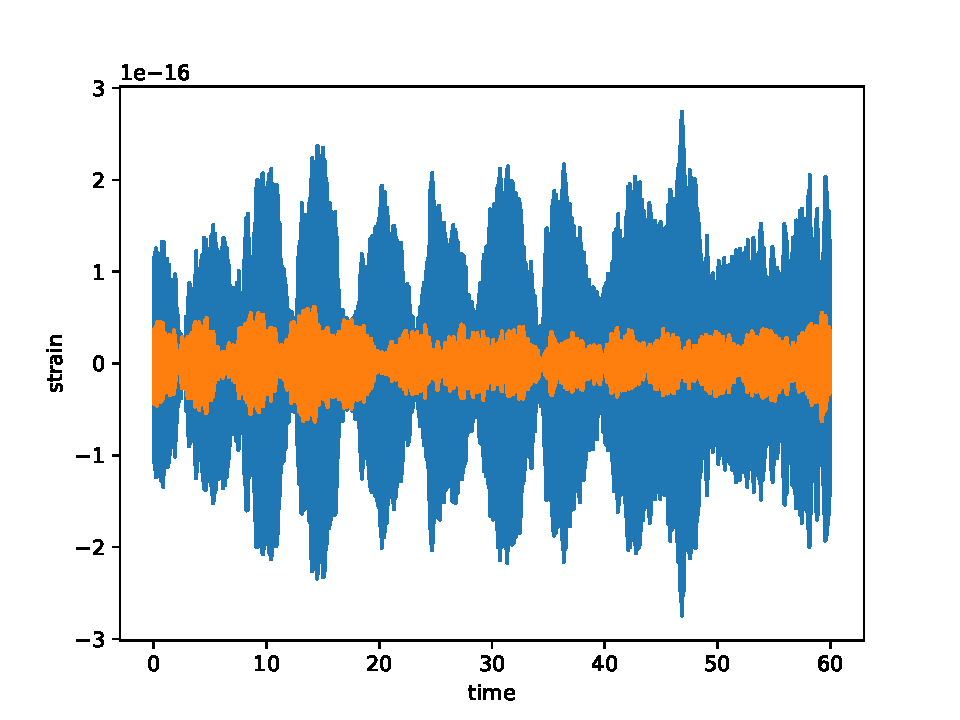
\includegraphics[width=\textwidth]{h1} \
				% remove the 'draft' keyword, when replacing with final figure!
				\caption{Signal in time}
			\end{figure}
		\column{0.5\textwidth}
			\centering
			\begin{figure}
				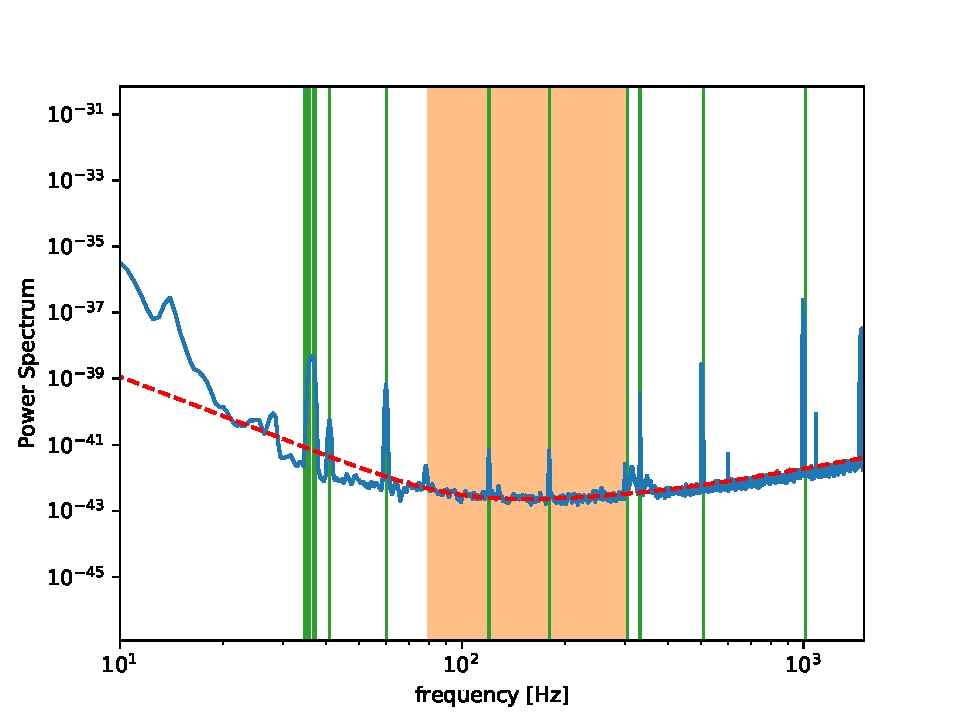
\includegraphics[width=\textwidth]{psd} \
				% remove the 'draft' keyword, when replacing with final figure!
				\caption{Power Spectrum Density}
			\end{figure}
		\column{0.0125\textwidth}
	\end{columns}
    \centering
    The measured strain is 
    \begin{equation}
    h = F_+(\bm{n}) \, h_+(\bm{n},f) + F_\times(\bm{n}) \, h_\times(\bm{n},f) 
        \end{equation}
	  \flushleft
      \footnotesize 
     $F_+$ and $F_\times$ are the \textbf{polarisation response functions} of the detector - depend on (lat,lon), pol. response, position of 		earth w.r.t. pol. basis $\Rightarrow$ $\bm{n} \equiv \bm{n}(t)$.\\
     \textcolor{white}{filler}\\
     \textcolor{white}{filler}
	%show data in t and f\\
    %show h = Fcross hcross + Fplus hplus
	%in each detector

\end{frame}

\begin{frame}
	\normalsize
	\frametitle{Correlating detecors, creating a beam on the sky}
		Correlate detectors to eliminate detector noise. Focus on GWB intensity $\bm{I}$ on the sky\\
    	$$I \propto \, <h_+\,h_{+}^{'\,\star}> + <h_\times\,h_{\times}^{'\,\star}>$$
        where $h_+(\bm{n}, f)$ and $h'_+\equiv h_+(\bm{n'}, f')$ from $\neq$ detectors.\\
        \medskip
        The combined response to $I$ of a single baseline (pair of dect.s) is
        \begin{equation}
        \gamma_{I,\,ab} (\bm{n}) =F^+_aF^{+\,\star}_b+F^\times_aF^{\times\,\star}_b\,
        \end{equation}
        $a$, $b$: dect. labels.\\
        \medskip
        
        %%% pol: quaternions
        \textbf{note}: $\neq$ pol. modes have $\neq$ \textbf{overlap functions}; we use \textbf{quaternions} to deal with geometry+polarisation.
        %\textcolor{red}{natural space: spherical harmonics}\\
    	%show how the gamma functions come about - don't lose too much time on stokes' parameters\\
		%show the gammaI gif;
    
\end{frame}

%     \begin{frame}
%     \frametitle{$\gamma_I$}
%         \transduration<0-9>{0}
%         \multiinclude[<+->][format=png, graphics={width=\textwidth}]{gammaI}
%     \end{frame}

{\setbeamercolor{background canvas}{bg=black!19!white}
\begin{frame}[plain]
\centering
\vskip 2cm
\includegraphics[width=0.95\textwidth]{bases/1b}
\vskip 2cm
\flushright
\tiny{\textcolor{white!50!black}{Image Credit: NASA}}

\end{frame}}

%%%%%%%%%%%%%%%%%%%%%%%%%%%%%%%%%%%%%%%

\begin{frame}

	\frametitle{$\gamma_I$}
    
	\begin{figure}
	  \animategraphics[loop,controls,width=0.8\linewidth]{8}{gammaI/gamma_rot}{0}{26} %26
		% remove the 'draft' keyword, when replacing with final figure!
	\caption{The overlap function $\gamma_I$ on the sky for the LIGO detector pair. The scale of the beam sets the reconstruction resolution. Note: peaked $\Rightarrow$ aliasing on large scales.}
	\end{figure}
    \smallskip

\end{frame}

{\setbeamercolor{background canvas}{bg=black!19!white}
\begin{frame}[plain]
\centering
\vskip 2cm
\includegraphics[width=0.95\textwidth]{bases/1b}
\vskip 2cm
\flushright
\tiny{\textcolor{white!50!black}{Image Credit: NASA}}

\end{frame}


\begin{frame}[plain]
\centering
\vskip 2cm
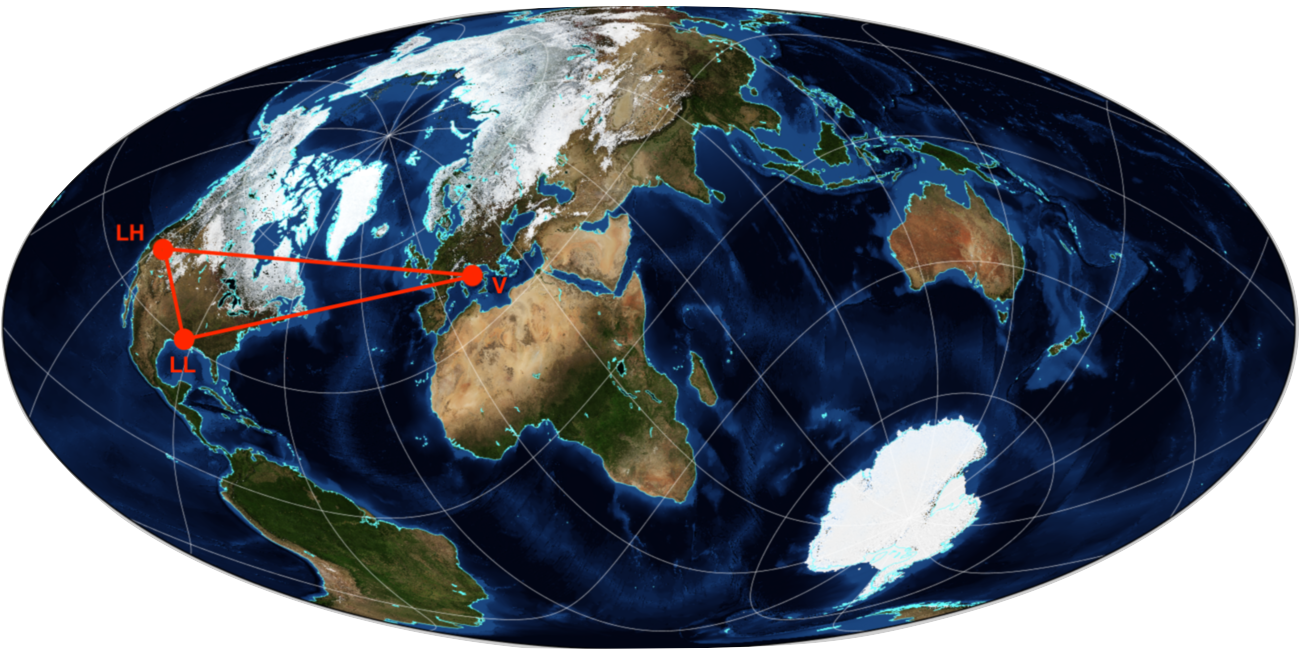
\includegraphics[width=0.95\textwidth]{bases/3b}
\vskip 2cm
\flushright
\tiny{\textcolor{white!50!black}{Image Credit: NASA}}

\end{frame}

\begin{frame}[plain]
\centering
\vskip 2cm
\includegraphics[width=0.95\textwidth]{bases/6b}
\vskip 2cm
\flushright
\tiny{\textcolor{white!50!black}{Image Credit: NASA}}

\end{frame}
\begin{frame}[plain]
\vskip 2cm
\centering
\includegraphics[width=0.95\textwidth]{bases/10b}\\
\vskip 1.1 cm
Larger network $\rightarrow$ larger coverage of the sky\\
\flushright
\tiny{\textcolor{white!50!black}{Image Credit: NASA}}

\end{frame}
}

\begin{frame}
	\frametitle{Noise-domination}
    \bigskip
    \medskip
    The correlated signal $<H_a\,H_b^{'\,\star}> \equiv d_t(\bm{b},f)$ is\footnote{if all anisotropies are 0. \\}
    \begin{equation}
d_t(\bm{b},f) =\delta_{\bm{n},\bm{n}'}\,\delta_{f,f'}\int_{S^2} d\bm{m}\, \gamma_{I,\,ab}(\bm{m})\,I(f,\,\bm{m})\,e^{2\pi i f \bm{m}\cdot\bm{b}}%(\bm{x_a}-\bm{x_b})}
% \star <arianna.renzini15@imperial.ac.uk> 2017-12-05T16:13:47.303Z:
%
% ^.
\label{corr}
\end{equation}
	this is dominated by gaussian random noise:
    \begin{equation}
	d_t(\bm{b},f) = s_t(\bm{b},f)+n_t(f)\,.
	\end{equation}
	
    \begin{block}{}
    $\Rightarrow$ \textbf{The PSD of the noise is just the PSD of the data:}
    \end{block}
	\begin{equation}
	<n_{t,\, a}(f)\,n_{t,\,b}^\star(f')> = \delta_{tt'}\delta_{ff'}N_{t,\,t'}(f, f')\,,
	\end{equation}
    $$
    \qquad N_{t,\,t'}(f,f') = P_{t,\, a}(f)P_{t',\, b}(f')\,, \qquad P_t(f) = <d_t(f)>^2.
    $$
    \medskip
    
    %%%%%%CHECK THIS!
    
    %Only the signal is directionally dependent $\Rightarrow$ we extract it.\\
    %\medskip
	%PSD of data $\equiv$ PSD of noise $\Rightarrow$ use as optimal weighting. \\
    %correlate between detectors to extract $d^T$
    %\textcolor{red}{maybe parallel with cmb @carlo?}\\
    
\end{frame}

%\begin{frame}
%	\frametitle{Noise-domination}
		
        
        
%\end{frame}

% \begin{frame}
% 	\frametitle{Making the map: spherical harmonics decomposition}
% 		\begin{equation}
% 			d_t(\bm{b}, f) = \int_{S^2}d\bm{m}\,I(\bm{m})\,\gamma_I(\bm{m})\,E(f)\,e^{2\pi i f\,\bm{b}\cdot\bm{m}}\,
% 		\end{equation}
%     	is the correlated data as a function of frequency $f$ and the \textbf{baseline} $\bm{b}(t)$; decompose it:
%         \begin{equation}
%         \begin{split}
%         	d_t(\bm{b}, f) = \sum_{lm}& d_{lm}^t(f) Y_{lm}^\star(\hat{b})\,,\\
% 			d_{lm}^t = 4\pi i^l F_l(b) \sum_{LM,L'M'}& a^I_{LM} \gamma^I_{L'M'} K_{LM,L'M',lm}\,.
% 			\label{dtlm}
%             \end{split}
% 		\end{equation}
        
%         $K_{LM,L'M',lm}$: coupling kernel. Summing over $(lm)$, $(L'M')$ we get
        
%         \begin{equation}
% 			 d_t(\bm{b}, f) = \sum_{LM} a^I_{LM} M^I_{LM}(\bm{b}, f)\,.
%             \label{dt}
% 		\end{equation}
%         \smallskip
% \end{frame}
%%%%%%%%%%%%%%%%%%%%%%%%%%%%%%%%%%%%

%\begin{frame}
%n is a direction => labels pixel number
%\end{frame}

%%%%%%%%%%%%%%%%%%%%%%%%%%AHAHAH

\begin{frame}
	\frametitle{Making the map: maximum likelihood map}

		Extract $\bm{I(m)}$ by minimizing the $\chi^2$ of the map given the data [Thrane et al, 2009]; defining the \textbf{dirty map} $z_{n}$:\\
        \small
        \begin{equation}
			z_{n} : = \sum_{T,\, f} \frac{M_{n}^{I\star}(\hat{b})}{N(f)} d^T(f, \hat{b})\,;
			\label{dirtym}
		\end{equation}
		\begin{equation}
			z_{n} = \sum_{m_{pix}} A_{mn}\,I_{m}\,, \,\,\,\,\,\,\, A_{mn} =  \sum_{T,\, f} 				\frac{M_{m}^I(\hat{b})M_{n}^{I^\star}(\hat{b}) }{N(f)}\,,
		\end{equation}
        \normalsize
and the map solution which maximizes likelyhood is 
\begin{block}{}
\begin{equation}
I_{m} = \sum_{n_{pix}}  \left(A_{mn}\right)^{-1} z_{n} \,.
\end{equation}
\end{block}
We call $I_{m}$ the \textbf{clean map} and $\bm{A}$ the \textbf{beam-pattern matrix}. 
\end{frame}

%%%%%%%%%%%%%%%%%%%%%%%%%

%%%%%%%%%%%%%%%%%%%%%%

\begin{frame}
	\frametitle{Making the map: what happens in the code}
Track time-coincident blocks of data in the dect.s and divide into equal segments, which are FFTd to get $d_{f}$; then:  
\begin{equation}
z_{n} = \sum_{T\in \text{ block}}\,\textcolor{green!70!black}{\sum_{b\,\in \,\text{base}}}\,\sum_{f\in F} M_{n,\,f_i}\,\tilde{d}_{f_i}\,, \qquad \tilde{d}_{f_i} = \delta_{ij}N^{-1}_{f_if_j}\,d_{f_j}\, , 
\end{equation}
$$\qquad  f_i,  f_j \in \tilde{T}=F =\{ f_1, f_2, f_3, ..., f_N\}\, .$$
Build $A_{mn}$ and invert it to extract the clean map $I_{m}$
\begin{equation}
 A_{mn} = \sum_{T\in \text{ block}} \,\textcolor{green!70!black}{\sum_{b\,\in\, \text{base}}}\,\sum_{f\in F} M^T_{m,\,f}\,N^{-1}_{ff}\,M^T_{n\,,f}\,,
\end{equation}
 $$
 I_{m} = A_{mn}^{-1} z_{n}\,,
 $$
which gets \textbf{accumulated over time}.
\end{frame}

%%%%%%%%%%%%%%%%%%%%%

% \begin{frame}
% 	\frametitle{What's in a map}
%     \vskip -5 mm
%     	\begin{figure}[h]
% 			\centering
% 			\includegraphics[width=0.75\textwidth]{S_p1}
% 			\scriptsize
% 			\caption{The output of the analysis of $\sim$ 2 days of LIGO S6 (2009-2010) open data. Unexciting as $\ell_{max} = 4$.}
% 			\label{output}
% 		\end{figure}
%         \vskip -5 mm
% 		We are still interpreting this... and inputting simulated data.
% \end{frame}

\begin{frame}
	\frametitle{Multiple baselines}
    	The beam-pattern matrix for 1 baseline isn't easily invertible, we've been relying on SVD techniques.\\
        \bigskip
        We need multiple baselines to break the singularity of the beam-pattern matrix, and scan the $uv$ space more 		efficiently. \\
        \bigskip
        The code allows an input from any number of detectors on earth - one just needs to simulate data from extra detectors 
        \bigskip
            \begin{block}{}
			Simple test: simulate correlated data for different baselines
    		\end{block}
\end{frame}

%%%%%%%%%%%%%%%%%%%%%%%%%
{\setbeamercolor{background canvas}{bg=black!19}
\begin{frame}[plain]
\centering
\includegraphics[width=0.95\textwidth]{bases/6b}


\end{frame}}

%%%%%%%%%%%%%%%%%%%%%%%%%


%may just drop this frame

\begin{frame}
	\frametitle{Correlated input maps}
	We simulate input maps by treating the signal and the noise separately;\\
    \medskip
    
    \begin{tabular}{>{\RaggedRight\arraybackslash}p{5.5em}>{\RaggedRight\arraybackslash}p{21em}}
  	\textcolor{blue}{input noise}: & take PSD of existing data and simulate gaussian \\
  	&  noise around it \\
    \vskip 1mm
    \textcolor{blue}{input signal}: &    \vskip 1mm create $I_m$ input signal and feed it into the\\
    & relevant baseline using Eq. (4) [Cornish, 2001]:\\
	\end{tabular}  

\[
d_t(\bm{b},f) =\delta_{\bm{n},\bm{n}'}\,\delta_{f,f'}\int_{S^2} d\bm{m}\, \gamma_{I,\,ab}(\bm{m})\,I(f,\,\bm{m})\,e^{2\pi i f \bm{m}\cdot\bm{b}}	%(\bm{x_a}-\bm{x_b})}
% \star <arianna.renzini15@imperial.ac.uk> 2017-12-05T16:13:47.303Z:
%
\]

	\textbf{Comparing input/output maps is key to testing the mapper.}
\end{frame}

% \begin{frame}
% \frametitle{Testing the mapper: the input map}
% We input the simple octupole, with 0 noise:
% \centering
% \includegraphics[width=0.75\textwidth]{8pole} \\
% and reconstruct it with the mapper...
% \end{frame}

% \begin{frame}
% \frametitle{Testing the mapper: reconstructing an input map}
% 	\begin{figure}
% 	  \animategraphics[controls,width=0.7\linewidth]{1}{map/S_p_}{1}{11} %26
% 		% remove the 'draft' keyword, when replacing with final figure!
% 	\caption{Result with 4 dect.s for 15h. Note: the noise in the image is just numerical noise from the inversion. They symmetry of the $\gamma$ makes this reconstruction easy...}
% 	\end{figure}
% \end{frame}
%%%%%%%%%%%%%%%%%%%%%%%%%%%%%%%%%

\begin{frame}
\frametitle{Next steps}
In bullet points:\\
\medskip
\begin{itemize}
\item Produce model-based input maps and test reconstruction
\item Include polarisation reconstruction
\item Test and interpret spherical harmonic response of the setup and the $\gamma_{eff}$
\item Use the new LIGO data \textbf{\textcolor{blue!50!white}{(just out!)}}
\item Generalize to other detector types: LISA
\end{itemize}
LISA is expected to probe extensively the frequency range for the AGWB... good news!
\medskip
\Large
\pause
\begin{center}
\textbf{\textcolor{blue}{Thanks for listening!}}
\end{center}
\end{frame}

\begin{frame}

\end{frame}

\begin{frame}
	\frametitle{Making the map: maximum likelihood map}

		The goal is to extract the $a^I_{LM}$. We do this by minimizing the 			$\chi^2$ of the map given the data [Thrane et al, 2009]:\\
        %\small
        \begin{equation}
		\chi^2(I_{m}) = -\frac{1}{2} \sum_{t,\,f}\frac{(d_t-<d_t>)(d_t-			<d_t>)^\star}{N(f)}
		\label{chisqu}
		\end{equation}
        $$\text{where}\quad d_t(f) = \, s^\star_{a,\,t}(f)\,s_{b,\,t}(f)\,, \qquad 	 <d_t(\bm{b}, f)>\equiv d_t(\bm{b}, f) .
 $$	%\frac{2}{\tau}
      %\textcolor{blue}{Notation: T labels data blocks; t labels time}\\
        $$
        \medskip
        \text{from (9)}: \quad \frac{\de \,<d_t(\bm{b},f)>}{\de\, I_{m}} = M_{m}^I(\bm{b})\,;
        $$
    then we carry out the calculations...
\end{frame}

%%%%%%%%%%%%%%%%%%%%%%%%%

\begin{frame}
	\frametitle{Making the map: maximum likelihood map}
    \smallskip
		Defining the \textbf{dirty map} $z_{m}$:
        \begin{equation}
			z_{m} : = \sum_{T,\, f} \frac{M_{m}^{I\star}(\hat{b})}{N(f)} d^T(f, \hat{b})\,;
			\label{dirtym}
		\end{equation}
		\begin{equation}
			z_{m} = \sum_{n} A_{mn}I_{n}\,, \,\,\,\,\,\,\, A_{mn} =  \sum_{T,\, f} 				\frac{M_{n}^I(\hat{b})M_{n}^{I^\star}(\hat{b}) }{N(f)}\,,
		\end{equation}
and the map solution which maximizes likelyhood is 
\begin{block}{}
\begin{equation}
I_{n} = \sum_{m}  \left(A_{mn}\right)^{-1} z_{m} \,.
\end{equation}
\end{block}
We call $I_m$ the \textbf{clean map} and $A$ the \textbf{beam-pattern matrix}. 
\end{frame}

% \begin{frame}
% 	\frametitle{Table and Block}
% 	\begin{table}[h]
% 		\centering
% 		\begin{tabular}{p{0.2\textwidth} p{0.7\textwidth}} 
% 			\toprule
% 			\multicolumn{2}{p{0.9\textwidth}}{TableTitle} \\
% 			\midrule
% 			CapA       & lots of examplesA \\

% 			CapB       & lots of examplesB \\
			
% 			CapC       & lots of examplesC \\
% 			\bottomrule
% 		\end{tabular} 
% 	\end{table}

% 	\begin{block}{BlockTitle}
% 		something to emphasise
% 	\end{block}
% \end{frame}


% \begin{frame}
% 	\frametitle{Two Figures aside}
% 	\begin{columns}[b]
% 		\column{0.0125\textwidth}
% 		\column{0.4875\textwidth}
% 			\centering
% 			\begin{figure}
% 				\includegraphics[draft,width=\textwidth]{fooA.pdf} \
% 				% remove the 'draft' keyword, when replacing with final figure!
% 				\caption{Caption of Figure A}
% 			\end{figure}
% 		\column{0.4875\textwidth}
% 			\centering
% 			\begin{figure}
% 				\includegraphics[draft,width=\textwidth]{fooB.pdf} \
% 				% remove the 'draft' keyword, when replacing with final figure!
% 				\caption{Caption of Figure B}
% 			\end{figure}
% 		\column{0.0125\textwidth}
% 	\end{columns}
% \end{frame}


% \begin{frame}
% 	\frametitle{Text and Figure aside}
% 	\begin{columns}[]
% 		\column{0.0125\textwidth}
% 		\column{0.4875\textwidth}
% 			\centering
% 			\begin{figure}
% 				\end{document}
\begin{frame}
	%\frametitle{Introduction: what is the GWB?}
    
    	\begin{figure}[h]
			\centering
			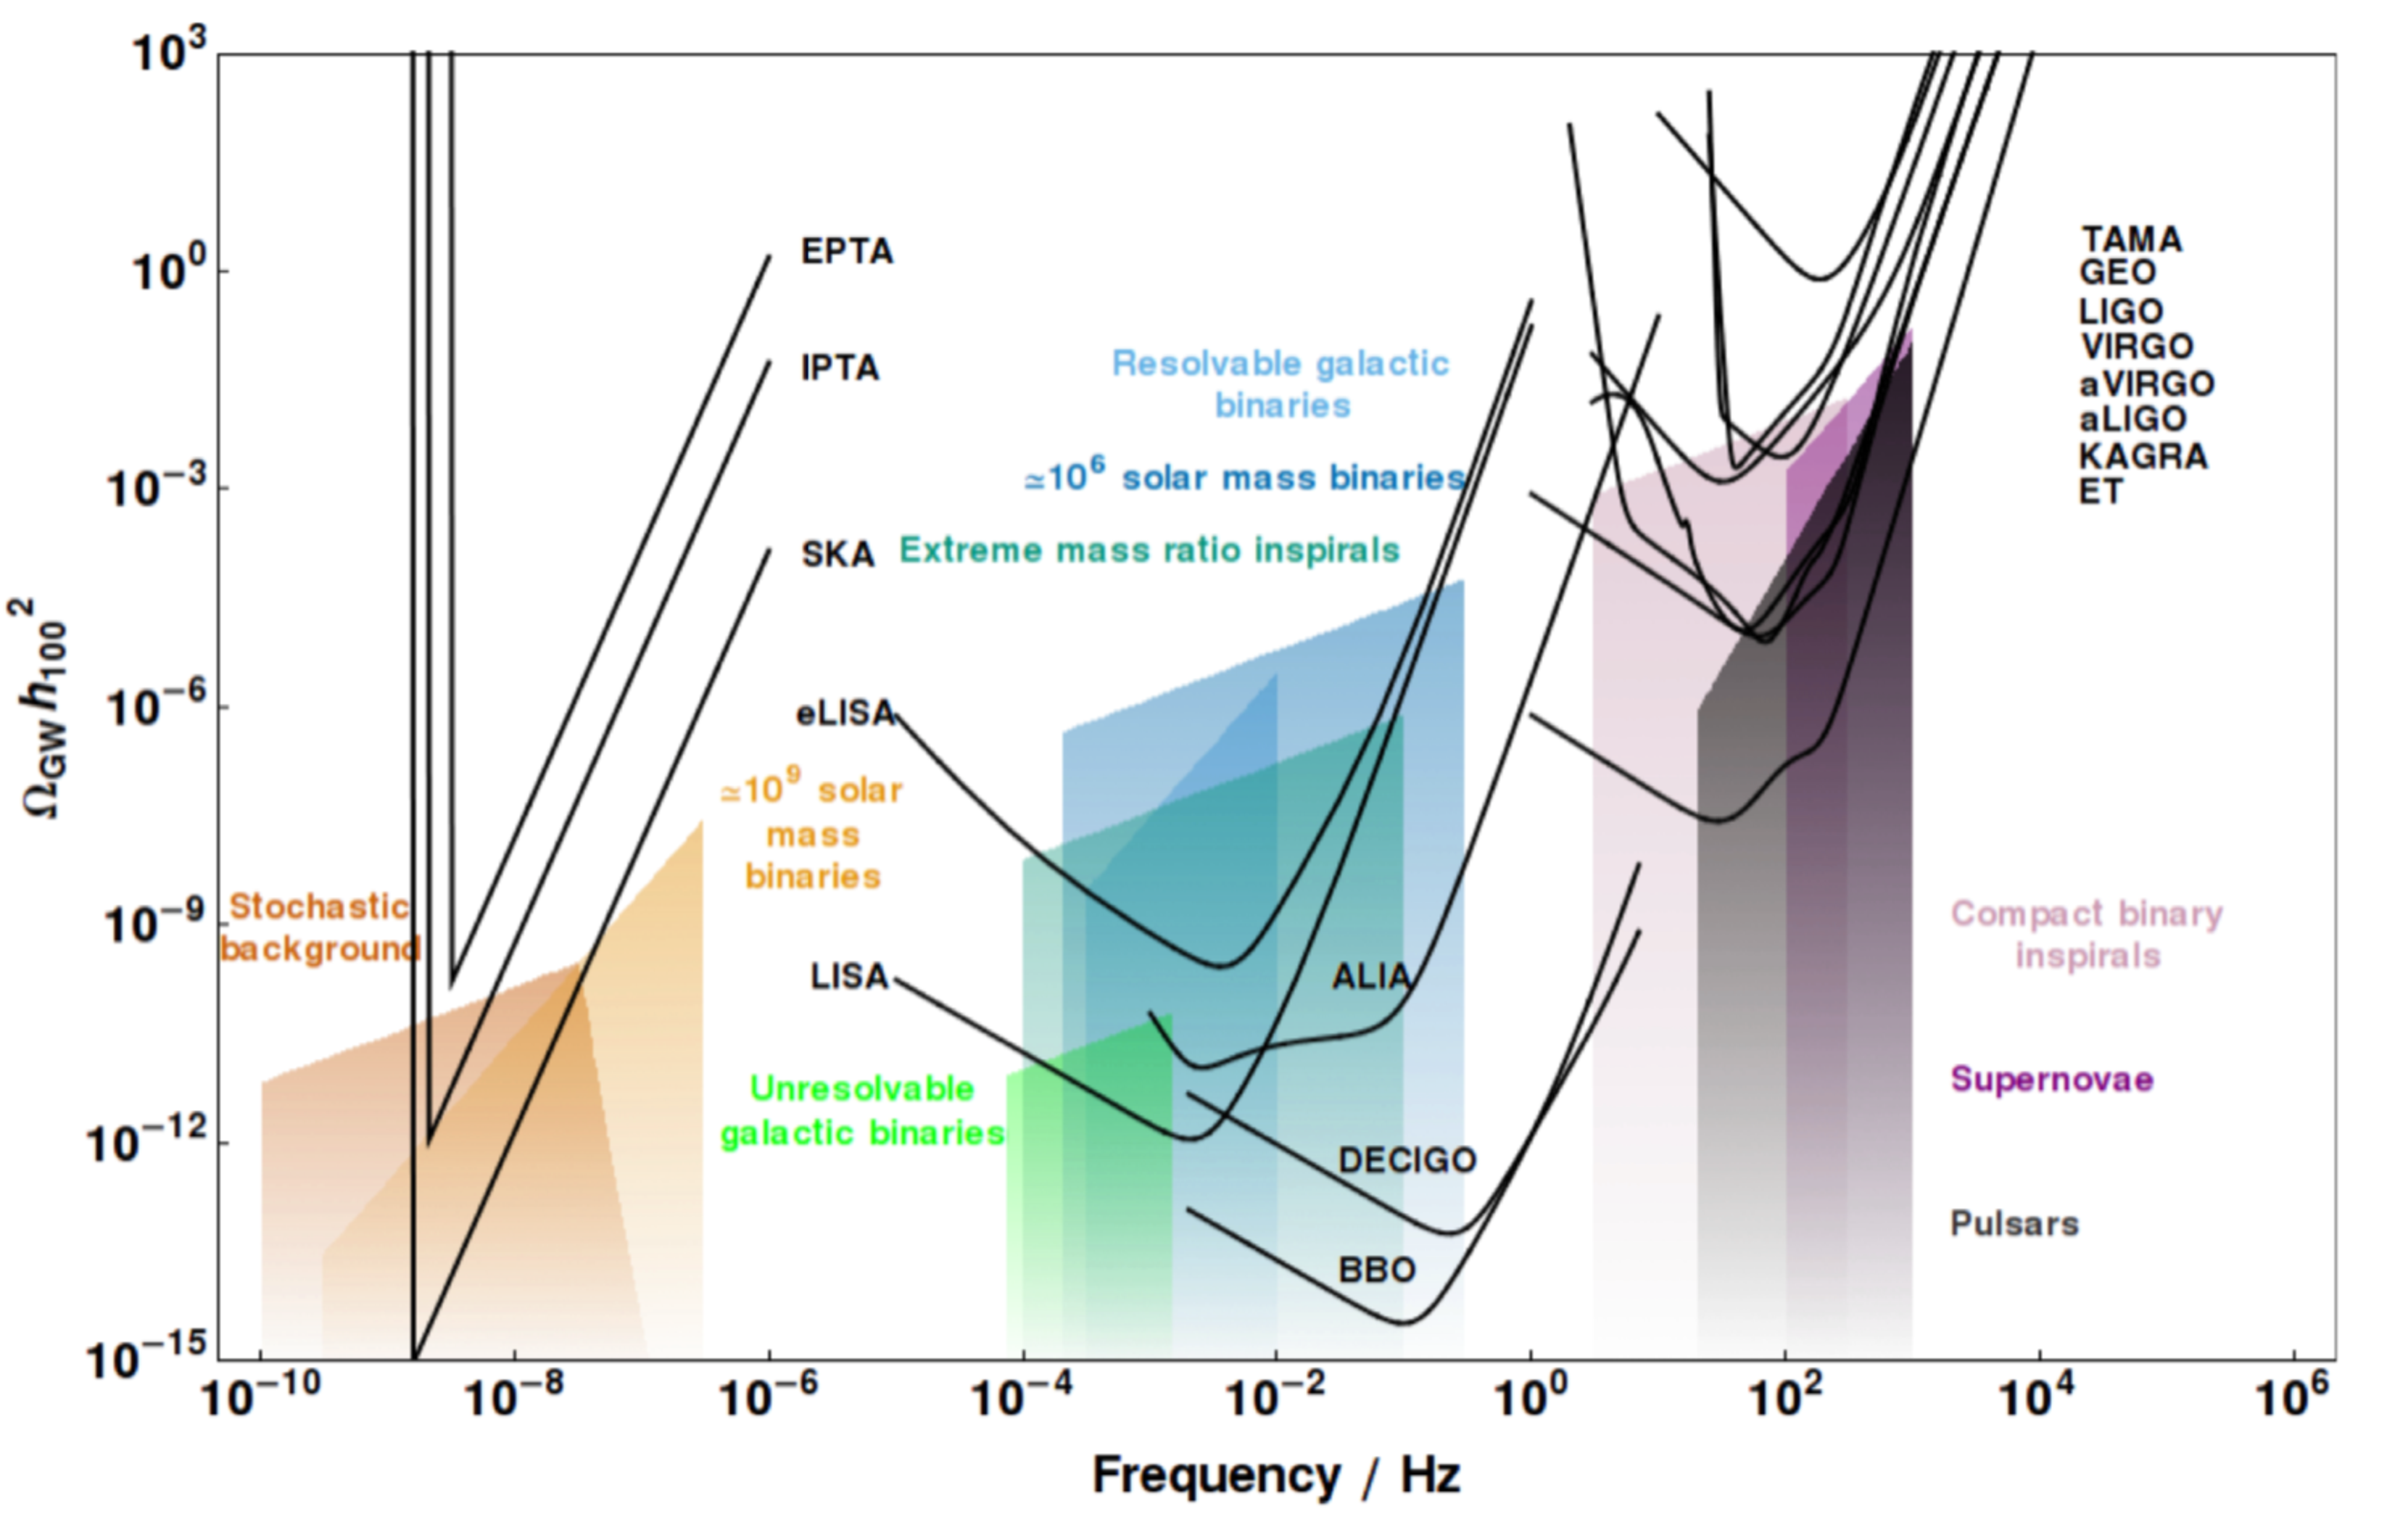
\includegraphics[width=0.95\textwidth]{GWBplots}
			\scriptsize
			\caption{Current constraints on the GWB and models, from [Moore et al., 2014].}
			\label{output}
		\end{figure}
\includegraphics[draft,width=\textwidth]{fooC.pdf} \
% 				% remove the 'draft' keyword, when replacing with final figure!
% 				\caption{Caption of Figure C}
% 			\end{figure}
% 		\column{0.4875\textwidth}
% 			Some text and a bullet point list
% 			\begin{itemize}
% 				\item ItemA
% 				\item ItemB
% 				\item ItemC
% 				\item ItemD
% 			\end{itemize}			
% 		\column{0.0125\textwidth}
% 	\end{columns}
\end{frame}


% \begin{frame}
% 	\frametitle{One Figure}
% 	\bigskip
% 	\begin{figure}
% 		\includegraphics[draft,width=0.8\textwidth, height=0.5\textwidth]{fooD.pdf}
% 		% remove the 'draft' keyword, when replacing with final figure!
% 		\caption{Caption of Figure D}
% 	\end{figure}
% \end{frame}

 \bibliographystyle{apalike}
\bibliography{9mbib}
\end{document}




